\section{Modelo de dados}

Uma das componentes importantes do desenho de um sistema de informação, passa por criar um modelo que explique as características de funcionamento e comportamento do \textit{software} a ser desenvolvido. A modulação para além de ajudar na compreensão do sistema, evita erros de programação, de projeto e de funcionamento.

\subsection{Modelo de Domínio}

Um dos primeiros passos na planificação do nosso sistema passou pela definição do \textbf{Modelo de Domínio}.
Podemos classificar como domínio do nosso sistema, o conjunto de características que descrevem a família de problemas que a nossa aplicação pretende solucionar.

Podemos consultar na Figura ~\ref{fig:modelo-dominio} os termos do nosso sistema e as relações existentes entre esses termos.

\begin{figure}[H] 
  \centering
  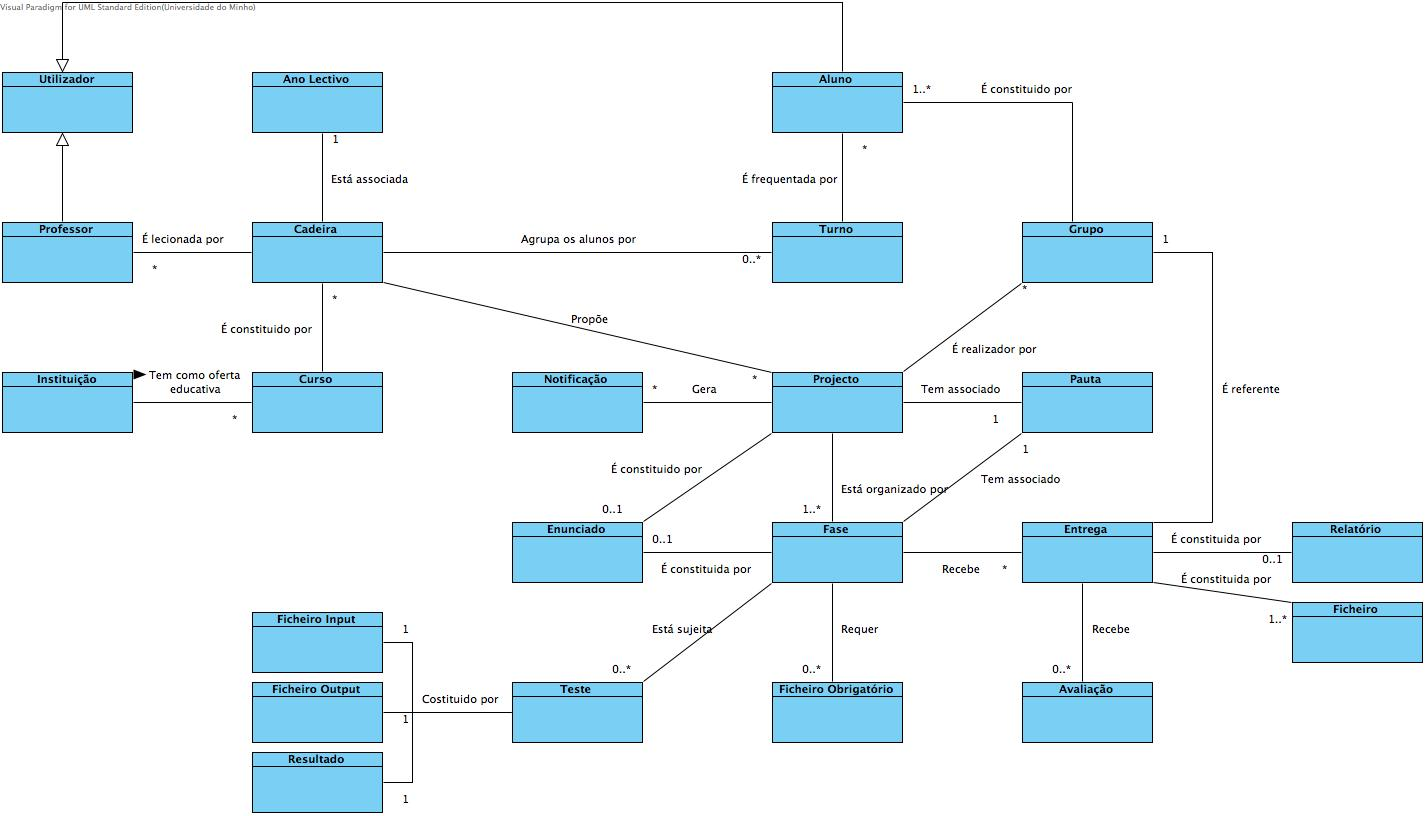
\includegraphics[width=1\textwidth,center]{images/modelo_dados/modelo-dominio}
  \caption{Modelo de domínio}
  \label{fig:modelo-dominio}
\end{figure}
